\documentclass[12pt]{article}
\usepackage{stmaryrd}
\usepackage{graphicx} % Pour l'insertion d'images
\usepackage{float}    % Pour contrôler précisément le placement
\usepackage[utf8]{inputenc}

\usepackage[french]{babel}
\usepackage[T1]{fontenc}
\usepackage{hyperref}
\usepackage{verbatim}

\usepackage{color, soul}

\usepackage{pgfplots}
\pgfplotsset{compat=1.15}
\usepackage{mathrsfs}

\usepackage{amsmath}
\usepackage{amsfonts}
\usepackage{amssymb}
\usepackage{tkz-tab}
\author{Destiné aux élèves de Terminale S\\Lycée de Dindéfelo\\Présenté par M. BA}
\title{\textbf{Rappels et compléments sur les fonctions numériques}}
\date{\today}
\usepackage{tikz}
\usetikzlibrary{arrows, shapes.geometric, fit}

% Commande pour la couleur d'accentuation
\newcommand{\myul}[2][black]{\setulcolor{#1}\ul{#2}\setulcolor{black}}
\newcommand\tab[1][1cm]{\hspace*{#1}}

\usepackage[margin=2cm]{geometry}
\usepackage{eso-pic}         % Pour ajouter des éléments en arrière-plan

\usepackage{enumitem}
%---------------------------------------
% Définir un compteur pour les exemples
\newcounter{exemple}

% Définir la commande \exemple pour afficher un exemple numéroté
\newcommand{\exemple}{%
  \refstepcounter{exemple}% Incrémenter le compteur
  \textbf{\textcolor{orange}{Exemple \theexemple : }} \ignorespaces
}
%---------------------------------------
\newcounter{solution}

% Définir la commande \solutione pour afficher un solution numéroté
\newcommand{\solution}{%
  \refstepcounter{solution}% Incrémenter le compteur
  \textbf{\textcolor{orange}{Solution \thesolution : }} \ignorespaces
}
%---------------------------------------
\definecolor{myorange}{rgb}{1.0, 0.8, 0.0}

% Définir un compteur pour les exercices d'application
\newcounter{exerciceapp}

% Définir la commande pour afficher un exercice d'application numéroté
\newcommand{\exerciceapp}{%
  \refstepcounter{exerciceapp}%
  \textbf{\textcolor{myorange}{Exercice d'application \theexerciceapp :}} \ignorespaces
}
%--------------------------------------
% Définir un compteur pour les exercices d'application
\newcounter{correction}

% Définir la commande pour afficher un correction exercice d'application numéroté
\newcommand{\correction}{%
  \refstepcounter{correction}%
  \textbf{\textcolor{myorange}{Correction \thecorrection :}} \ignorespaces
}
%--------------------------------------
% Définir un compteur pour les remarque d'application
\newcounter{remarque}

%----------------------------------------
\definecolor{myorange1}{rgb}{1.0, 1.5, 0}
% Définir la commande pour afficher un remarque numéroté
\newcommand{\remarque}{%
  \refstepcounter{remarque}%
  \textbf{\textcolor{myorange1}{Remarque \theremarque :}} \ignorespaces
}
% Commande pour ajouter du texte en arrière-plan
\AddToShipoutPicture{
    \AtTextCenter{%
        \makebox[0pt]{\rotatebox{45}{\textcolor[gray]{0.9}{\fontsize{5cm}{5cm}\selectfont Pathé BA}}}
    }
}

\begin{document}
\maketitle
\section*{\underline{\textbf{\textcolor{red}{A. LIMITES ET CONTINUITÉ}}}}
\subsection*{\underline{\textbf{\textcolor{red}{I.Limites}}}}

\renewcommand{\labelenumi}{\theenumi)}
\begin{enumerate}[label=\arabic*)]
    \item \textbf{\textcolor{blue}{\underline{Quelques limites usuelles}}}
    
\[\forall n\in\mathbb{N}^{*} \lim_{x \to +\infty} x^{n}=+\infty  \text{ , } \lim_{x \to +\infty} \frac{1}{x^{n}}=0^{+}  \]

\[ \forall n\in\mathbb{N}^{*}
 \lim_{x \to -\infty} x^{n} =
 \begin{cases} 
 +\infty \text{ si \(n\) est pair}\\
 -\infty \text{ si \(n\) est pair}
 \end{cases}
\text{ , }
\lim_{x \to -\infty} \frac{1}{x^{n}}=
 \begin{cases} 
 0^{+} \text{ si \(n\) est pair}\\
 0^{-} \text{ si \(n\) est pair}
 \end{cases}
\]

\[ \lim_{x \to +\infty} \sqrt{x}=+\infty \text{ , } \lim_{x \to +\infty} \frac{1}{\sqrt{x}}=0^{+}  \]

\[ \lim_{x \to a^{+}} \frac{1}{x-a}=+\infty \text{ , } \lim_{x \to a^{-}} \frac{1}{x-a}=-\infty  \]

		\textbf{Autre Notation}
\[( x\rightarrow a^{+} ) \Leftrightarrow ( x\rightarrow a_{>} ) \text{ , } ( x\rightarrow a^{-} ) \Leftrightarrow ( x\rightarrow a_{<} ) \]
\[ \lim_{x \to a^{+}} f(x)=+\infty \text{ se note aussi } \lim_{x \to a_{>}} f(x)=+\infty  \]	

\[ \lim_{x \to a^{-}} f(x)=-\infty \text{ se note aussi } \lim_{x \to a_{<}} f(x)=-\infty  \]	
    
    \item	\textbf{\textcolor{blue}{\underline{Quelques théorèmes sur les limites}}}
\begin{enumerate}[label=\alph*)]
       \item \textcolor{green}{\underline{Théorème de comparaison}}
       
Soient \( f \) et \( g \) trois fonctions définies sur un intervalle \( I \) au voisianage \( \alpha \), \( \alpha \) étant un réel, \( +\infty \) ou \( -\infty \).

\[ \text{Si pour tout \( x\in  I \): }
  \begin{cases}
    f(x)\geq g(x)\\
    \lim_{x \to \alpha}g(x)=+\infty 
  \end{cases}
\text{ alors }  \lim_{x \to \alpha}f(x)=+\infty 
\]

\begin{figure}[H]% Forcer l'image à cet endroit
\centering
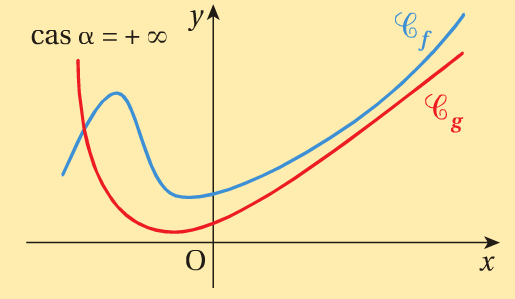
\includegraphics[width=0.8\textwidth]{comp1.png}
\caption{Courbe de (Cf)}
\label{fig:monimage}
\end{figure}

\[ \text{Si pour tout \( x\in  I \): }
  \begin{cases}
    f(x)\leq g(x)\\
    \lim_{x \to \alpha}g(x)=-\infty 
  \end{cases}
\text{ alors }  \lim_{x \to \alpha}f(x)=-\infty 
\]

\begin{figure}[H]% Forcer l'image à cet endroit
\centering
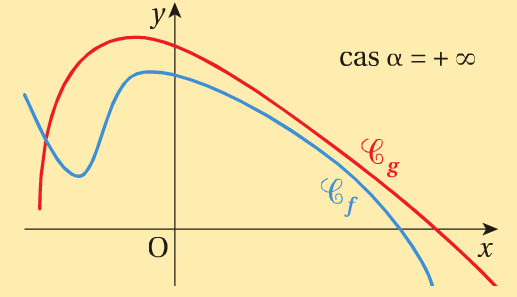
\includegraphics[width=0.8\textwidth]{comp2.png}
\caption{Courbe de (Cf)}
\label{fig:monimage}
\end{figure}

       	\textbf{\underline{\exemple:}}
       	\[ \text{Soit \( f(x)=-x+\sin x \) Calculer }\lim_{x \to +\infty} f(x) \]
       	
       	\newpage
       	\textbf{\underline{\solution:}}
       	\[ \text{Pour tout \(x\), \( \sin x\leq 1 \implies -x + \sin x \leq 1 - x \implies f(x)\leq 1 - x \).} \]
       	\[	\text{Posons \( g(x)=1-x \) donc \( f(x)\leq g(x) \).} \]
       	\[ \text{Or,} \lim_{x \to +\infty}g(x)=-\infty, \text{donc} \lim_{x \to +\infty}f(x)=-\infty\]       	
       	
       	 \textbf{\underline{\exemple:}}
       	\[ \text{Soit \( g(x)=\frac{\sqrt{1+x^{2}}}{x^{2}} \). Calculer }\lim_{x \to 0} g(x) \]
       	 \textbf{\underline{\solution:}}
       	 \[ \text{Posons \( f(x)=\frac{1}{x^{2}} \). Comme, pour tout \(x\neq 0\), on a, \( 1\leq \sqrt{1+x^{2}} \)., on a, pour tout }, x\neq 0 \]
       	\[ f(x)\geq g(x) \text{ Or,} \lim_{x \to 0}g(x)=+\infty, \text{donc} \lim_{x \to 0}f(x)=+\infty\]
       	
       	\item \textcolor{green}{\underline{Théorème d’encadrement ou théorème des gendarmes}}
       	
Soient \( f \), \( g \) et \( h \) trois fonctions définies sur un intervalle \( I \) au voisianage \( \alpha \), \( \alpha \) étant un réel, \( +\infty \) ou \( -\infty \).

Si \( \forall x\in I \quad g(x) \leq f(x)\leq h(x) \) et \( \lim_{x \to \alpha}g(x)=\lim_{x \to \alpha}h(x)=\ell,\) alors \( \lim_{x \to \alpha}f(x)=\ell \)
       	
       	\textbf{\underline{\exerciceapp}}
\[\text{ Calculer } \lim_{ x\to +\infty} \frac{x-\sin x}{x^{2}} \]   	
       	\textbf{\underline{\correction}}
       	
\item \textcolor{green}{\underline{Limite et composition de fonctions}}

Soit \( \alpha \), \( \beta \) et \( \gamma \) des réels ou \( \pm\infty \) On considère deux fonctions \( u \) et \( v \) telles que
\begin{itemize}
\item[•] \( \lim_{x \to \alpha}u(x)=\beta  \)
\item[•] \( \lim_{x \to \beta}v(x)=\gamma \)
\end{itemize}

Alors \( \lim_{x \to \alpha}v(u(x))=\gamma \) 	
	
       	\textbf{\underline{\exerciceapp}}	
\[\text{Calculer }\lim_{x \to +\infty}\sqrt{\frac{9}{x}+7} \]

				\textbf{\underline{\correction}}
				
On commence par la fonction la plus à l'intérieur :

\[\text{Posons } u(x)=\frac{9}{x}+7 \text{ et } v(x)=\sqrt{\frac{9}{x}+7} \]
       	\item \textcolor{green}{\underline{Théorème du changement de variable}}
       	\[ \lim_{x \to x_{0}}f(x)=f(x_{0}+t) \]
      	\[ \lim_{x \to +\infty}f(x)=\lim_{X \to 0^{+}}f \left( \frac{1}{X} \right)  \]
       	\[ \lim_{x \to -\infty}f(x)=\lim_{X \to 0^{-}}f \left( \frac{1}{X} \right)  \]
       	\textbf{Preuve[Exercice]}    	
			       		
      	\textbf{\underline{\exerciceapp}}

				 \[ \lim_{x \to +\infty}x\sin \frac{1}{x} \] 
				 \[ \lim_{x \to +\infty}x\tan \frac{3}{x} \] 
				 \[ \lim_{x \to +\infty}x^{2}\left( 1 - \cos \frac{2}{x} \right) \] 	

				\textbf{\underline{\correction}}       	

\item \textcolor{green}{\underline{Limites des fonctions trigonométriques}}      
       	\begin{itemize}
       	\item \[ \lim_{x \to 0} \frac{\sin x}{x}=1 \]
       	\item \[ \lim_{x \to 0} \frac{\tan x}{x}=1 \]
       	\item \[ \lim_{x \to 0} \frac{1-\cos x}{x^{2}}=\frac{1}{2} \]
       	\item \[ \lim_{x \to 0} \frac{\cos x -1 }{x}=0 \]
       	\end{itemize}
\end{enumerate}

\item \textbf{\textcolor{blue}{\underline{Interprétations géométriques des limites}}}

Les limites peuvent être interprétées géométriquement de plusieurs manières en fonction du contexte. Voici quelques exemples typiques :

\begin{enumerate}[label=\alph*)]
   \item \textcolor{green}{\underline{\textbf{Asymptote horizontale (AH)[Parllèle à \((ox)\)]}}}:
    
    Une fonction \( f \) a une asymptote horizontale en \( y = L \) lorsque
\[
\lim_{x \to +\infty} f(x) = L \text{ on dit que: \( y = L \) est une AH à \( (C_{f}) \) en }+\infty
\]
    
\[
\lim_{x \to -\infty} f(x) = L \text{ on dit que: \( y = L \) est une AH à \( (C_{f}) \) en }-\infty
\]
    
    Cela signifie que la courbe de la fonction se rapproche de la droite \( y = L \) à mesure que \( x \to +\infty \) ou \( x \to -\infty \).
    
\textbf{\underline{\exemple:}}

Déterminer l'AH de \( f \)
\[
    f(x) = \frac{2x^2}{x^2 + 1}
\] 
\textbf{\underline{\solution:}}
\[
\lim_{x \to +\infty} f(x) = 2, \quad \lim_{x \to -\infty} f(x) = 2.
\]
    La courbe de la fonction se rapproche de la droite \( y = 2 \) à mesure que \( x \to +\infty \) ou \( x \to -\infty \).
    \item \textcolor{green}{\underline{\textbf{Asymptote verticale (AV)[Parllèle à \((oy)\)]}}} :
    
    Soit \( x = a \in \mathbb{R} \) 
    \[
    \text{si }\lim_{x \to a} f(x) = \pm\infty \text{ alors \(x = a\) est une AV à \(C_{f}\)}
    \]
    Cela signifie que la courbe de la fonction tend vers l'infini lorsque \( x \) approche \( a \) par la droite (ou la gauche).

\textbf{\underline{\exemple:}}

Déterminer de l'AV de \( f \) tel que
\( f(x) = \frac{1}{x} \)

\textbf{\underline{\solution:}}
\[
\lim_{x \to 0^{+}} f(x) = +\infty \quad \text{et} \quad \lim_{x \to 0^{-}} f(x) = -\infty,
\]
ce qui signifie que la fonction a une asymptote verticale en \( x = 0 \).
    \item \textcolor{green}{\underline{\textbf{Asymptote oblique (AO)}}} :
\[ \text{Si } \lim_{x \to +\infty} (f(x)-(ax+b)) = 0 \text{ alors \(y = ax+b\) est une AO à \((C_{f})\) en \( +\infty \)} \]
\[  \]
\[ \text{Si } \lim_{x \to -\infty} (f(x)-(ax+b)) = 0 \text{ alors \(y = ax+b\) est une AO à \((C_{f})\) en \( -\infty \)} \]
\[  \]
Cette méthode est utilisée pour montrer que \(y=ax+b\) est est une AO

\textbf{\underline{\exemple:}}

Soit \( f \) une fonction et \( (C_{f}) \) sa courbe représentative.

Montrer que \( y = x + 2 \) est AO à \( (C_{f}) \) en \( \pm\infty \)

\textbf{\underline{\solution:}}

\( y = x + 2 \) est AO à \( (C_{f}) \) en \( \pm\infty \) si
\(\lim_{x \to +\infty}\left[ f(x)-y\right] =0 \)

En effet
    \[
    f(x) = \frac{x^2 + 2x + 1}{x}, \quad \lim_{x \to +\infty} \left( f(x) - (x + 2) \right) = 0.
    \]
    La courbe de la fonction se rapproche de la droite \( y = x + 2 \) pour \( x \to +\infty \).
\item \textcolor{green}{\underline{\textbf{Propriété 1[Autre façon de montrer que \( y = ax + b \) est une AO]}}}

Soit \( f \) une fonction, \( a, b \) un réel et \( (C_{f}) \) sa courbe représentative .
\[
\text{Si }\lim_{x \to +\infty}f(x)=\pm\infty 
\text{ et }
\lim_{x \to +\infty}\frac{f(x)}{x}=a
\text{ et }
\lim_{x \to +\infty}\left( f(x)-ax\right) =b
\]

\[
\text{ alors }
y = ax + b \text{ est une AO à } (C_{f}) en +\infty.
\]
\textbf{\underline{NB:}}

Cette propriété reste valable lorsque \( x\rightarrow -\infty\)

On aura \( y = ax + b \) est une AO à \( (C_{f}) \) en \(-\infty\)

\textbf{\underline{\exerciceapp}}

\begin{enumerate}[label=\arabic*)]

\item Soit \( f(x)=\frac{2x}{\sqrt{x+1}} \)
Déterminer \(Df\) et  montrer que \(x=-1\) est une AV à \( (C_{f}) \).

\item Soit \( g(x)=\sqrt{4x^{2}+1}+2x \)

	\begin{enumerate}[label=\alph*)]
		\item Montrer que \(y = 0\) est une AH à \( (C_{g}) \) en \(-\infty\) 
		\item Montrer que \(y = 4x\) est une AO à \( (C_{g}) \) en \(+\infty\) 
	\end{enumerate}

\end{enumerate}
\textbf{\underline{\correction}}

\item \textcolor{green}{\underline{Branche parabolique de direction (oy)}}
\[
 \text{Si } \lim_{x \to +\infty} f(x) = \pm\infty \text{ et } \lim_{x \to +\infty} \frac{f(x)}{x} = \pm\infty 
 \]
 
\[
\text{ alors \((C_{f})\) admet une branche parabolique de direction  \((oy))\) en \( +\infty \)} 
 \]
		\textbf{\underline{\remarque}}		

Cette propriété reste valable lorsque 	\(x \rightarrow -\infty\)	
		
\item \textcolor{green}{\underline{Branche pparabolique de direction (ox)}}
\[
 \text{Si } \lim_{x \to +\infty} f(x) = \pm\infty \text{ et } \lim_{x \to +\infty} \frac{f(x)}{x} = 0 
 \]
 
\[
\text{ alors \((C_{f})\) admet une branche parabolique de direction  \((ox))\) en \( +\infty \)} 
 \]
		\textbf{\underline{\remarque}}	
				
Cette propriété reste valable lorsque 	\(x \rightarrow -\infty\)	

\item \textcolor{green}{\underline{Branche parabolique de direction \(y = ax\) (a réel)}}
\[
 \text{Si } \lim_{x \to +\infty} f(x) = \pm\infty \text{ et } \lim_{x \to +\infty} \frac{f(x)}{x} = a \text{ et } \lim_{x \to +\infty} (f(x)-ax) = \pm\infty
 \]
 
\[
\text{ alors \((C_{f})\) admet une branche parabolique de direction  \(y=ax\) en \( +\infty \)} 
\]
		\textbf{\underline{\remarque}}	
				
Cette propriété reste valable lorsque 	\(x \rightarrow -\infty\)	
	
\textbf{\underline{\exerciceapp}}

Étudier les branches infinies des courbes représentatives des courbes des fonctions suivantes :
\begin{enumerate}[label=\alph*)]
\item \( f(x)=\frac{2x^{3}-1}{x-1} \)

\item \( g(x)=\sqrt{x^{2}+1}-x \)

\item \( h(x)=x\sqrt{\frac{x+1}{x-1}}\)
\end{enumerate}
\textbf{\underline{\correction}}

\end{enumerate}
		
\end{enumerate}

\subsection*{\underline{\textbf{\textcolor{red}{II.Continuité et  Dérivabilité}}}}

\begin{enumerate}[label=\arabic*)]
\item \textbf{\textcolor{blue}{\underline{Définition}}}

Soit f une fonction definie en \( x_{0} \) on dit que f est continue en \( x_{0} \) si
\( \lim_{x \to x_{0}} f(x)=f(x_{0}) \).

\begin{center}
\underline{\textbf{\textcolor{red}{Revoir}}}
\end{center}

\(\left[
\textbf{\textcolor{red}{\underline{Continuité à gauche et continuité à droite}}} 
\right] \)
			
\(\left[ 
\textbf{\textcolor{red}{\underline{Continuité à gauche et continuité à droite}}} 
\right] \)

\(\left[ 
\textbf{\textcolor{red}{\underline{Prolongement par continuité}}}	
\right] \) 

\(\left[ 		
\textbf{\textcolor{red}{\underline{Continuité sur un intervalle}}}
\right] \) 

\(\left[
\textbf{\textcolor{red}{\underline{Continuité de fonctions usuelles}}}
\right] \)

\(\left[
\textbf{\textcolor{red}{\underline{Opérations sur les fonctions continues}}}
\right] \)
\item \textbf{\textcolor{blue}{\underline{Compositions de deux fonctions continues}}}

Si \( f \) est continue en \(x_{0}\) et \( g \) est continue en \( f(x_{0}) \) alors \( gof \) est continue en \(x_{0}\) donc la composition de deux fonctions continues est une fonction continue.

		\textbf{\underline{\exerciceapp}}

		\begin{enumerate}[label=\alph*)]
			\item Soit 	\( f(x)=\sqrt{|2x^{5}|} \)		

		  	Etudier la continuité de 	\( f \) sur \( \mathbb{R} \)
		  
		 	\item Soit \( f(x)=x\sqrt{1-x} \)
		 
		 		Etudier la continuité de f sur son domaine de définition.
		\end{enumerate}	

		\textbf{\underline{\correction}}

\item \textbf{\textcolor{blue}{\underline{Image d’un intervalle par une fonction continue et stritement monotone}}}
\begin{itemize}
\item L’image d’un intervalle par une fonction continue est un intervalle.
\[
\text{C’est à dire}
\begin{cases}
\text{\( f \) est continue sur \( I \)}\\
\text{\( I \) est un intervalle}
\end{cases}
\text{alors \( f(I) \) est un intervalle}
\]

\item Lorsqu’une fonction \( f \) est continue et strictement monotone sur \( K \), \( f(K) \) est un intervalle de même nature que \( K \) et ses bornes sont les limites de \( f \) aux bornes de \( K \).

Le tableau ci-dessous précise \( f(K) \) suivant la nature de \( K \) et le sens de variation de \( f \).
\end{itemize}
\begin{tabular}{|c|c|c|c|}
\hline
\( K \) & \( f(K) \) & \( f(K) \)\\
\hline
				& \( f \) stictement croissante & \( f \) strictement décroissante\\
\hline
[a;b]		& \( [f(a);f(b)] \) & \( [f(b);f(a)] \)       \\
\hline
[a;b[	& \( [f(a);\lim_{x\to b^{-}}f(x)[ \) &	\( [\lim_{x\to b^{-}}f(x);f(a)[ \)	\\
\hline
]a;b[		& \( ]\lim_{x\to b^{+}}f(x);\lim_{x\to b^{-}}f(x)[ \) &	\( ]\lim_{x\to b^{-}}f(x);\lim_{x\to b^{+}}f(x)[ \)	\\
\hline
\( [a;+\infty[ \)	& \( [f(a);\lim_{x\to +\infty}f(x)[ \) &\( [\lim_{x\to +\infty}f(x);f(a)[ \)		\\
\hline
\( \mathbb{R} \)& \( ]\lim_{x\to -\infty}f(x);\lim_{x\to +\infty}f(x)[ \)&\( ]\lim_{x\to +\infty}f(x);\lim_{x\to -\infty}f(x)[ \)\\
\hline
\end{tabular}

			\textbf{\underline{\exerciceapp}}
			
				Soit \( f(x)=\frac{2x+1}{x-1} \)
				
				Déterminer l’image par \( f \) des intervalles \( [-2;0] \) et \( ]1;+\infty[ \)
				
			\textbf{\underline{\correction}}
			
\item \textbf{\textcolor{blue}{\underline{Théorème des valeurs intermediaries}}}

Si la fonction \( f \) est \textcolor{red}{ continue }  sur \( [a ; b] \) et si le réel \( m \) est compris entre \( f(a) \) et \( f(b) \), alors l'équation \( f(x) = m \) admet \textcolor{red}{ au moins } une seule solution dans \( [a ; b] \).

Autrement dit, il existe \textcolor{red}{ au moins } un réel \textcolor{red}{ c } entre \textcolor{red}{ \( a \) } et \textcolor{red}{ \( b \) } tel que \textcolor{red}{ \( f(c) = m \) }

\textbf{\textcolor{blue}{\underline{Ilustration graphique}}}

[Image]

\textbf{\underline{\exemple:}}

Soit la fonction \( f(x)=\frac{1}{2}x^{3}+x-5 \) continue sur \( [-2 ; 4] \).

\textbf{\underline{\solution:}}

\(f( [-2 ; 4] ) = [\lim_{x \to -2} f(x) ; \lim_{x \to 4} f(x)] = [-8,6 ; 11,8] \).

D'après le théorème précédent, comme  \(5\in [-8,6 ; 11,8] \) donc l'équation \( f(x) = 5 \) a une solution dans \( [-2 ; 4] \).

\textbf{\textcolor{blue}{\underline{NB}}}

\begin{itemize}
\item Si \(  m = 0 \) il suffit montrer que \( \lim_{x \to a} f(x) \times \lim_{x \to b} f(x) <0 \)
\item Il faut toujours commencer par montrer que \( f \) est continue.
\end{itemize}

\textbf{\underline{\exerciceapp}}

\( f(x) = 2x^{5} + x^{2} + x + 8 \)

Montrer que l’équation \( f(x) = 0 \) admet au moins une solution dans \( [1 ; 2] \).

\textbf{\underline{\correction}}

\item \textbf{\textcolor{blue}{\underline{Théorème d’existence et d’unicité d’une solution}}}

Si la fonction \( f \) est \textcolor{red}{ continue } et \textcolor{red}{ strictement monotone } (croissante ou bien décroissante) sur \( [a ; b] \). Pour tout réel \( m \) compris entre \( f(a) \) et \( f(b) \), alors l'équation \( f(x) = m \) admet une \textcolor{red}{unique continue } dans \(\alpha\in [a ; b] \).

\textbf{\textcolor{blue}{\underline{Ilustration graphique}}}

[Image]

\textbf{\textcolor{blue}{\underline{Cas particulier}}}

Si la fonction \( f \) réalise une bijection(continue et strictement monotone) de \( [a ; b] \) de plus si \( f(a) \times f(b) < 0 \) alors l'équation \( f(x) =0 \) admet une unique solution \( \alpha \) sur l'intervalle 
\( [a ; b] \).
\textbf{\textcolor{blue}{\underline{Ilustration graphique}}}

[Image]

			\textbf{\underline{\exemple:}}
			
			Soit \( f(x)=x^{3} + x + 1 \)

			Montrer que l’équation \( f(x) = 0 \) admet une unique solution sur \( [-0,8 ; -0,6] \).			
			
			\textbf{\underline{\solution:}}

\item \textbf{\textcolor{blue}{\underline{Théorème d’existence d’une bijection}}}

Si \( f \) est continue et strictement monotone sur un intervalle \( I \) alors \( f \) est une bijection de \( I \) vers \( J = f(I) \).

			\textbf{\underline{\exemple:}}
			
			Soit \( f(x) = x^{3} + x^{2} + x + 1 \)
			
			Montrer que \( f \) est une bijection de \( \mathbb{R} \) vers un intervalle \( J \) à préciser.			
			
			\textbf{\underline{\solution:}}
			
			\( f \) est une fonction polynôme donc elle est continue et dérivable sur \( \mathbb{R} \).(1)
			
			\( f'(x) = 3x^{2} + 2x + 1 \) 
			
			Etudions le signe de \( f' \) 
			
			Posons \( 3x^{2} + 2x + 1 =0  \)
			
			 \( \Delta' < 0 \) donc \( \forall x\in \mathbb{R}, f'(x) > 0\)
			 
			 D’où \( f \) est strictement croissante sur \( \mathbb{R} \).(2)
			 
			 D’après (1) et (2), \( f \) est une bijection de \( \mathbb{R} \) vers \( f(IR) = IR \)

			\textbf{\underline{\exerciceapp}}

			Trouve un exercice complet reunissant tous les théorème cités plus haut		
			
			\textbf{\underline{\correction}}

\item \textbf{\textcolor{blue}{\underline{Encadrement de la racine \( \alpha \) à \( \epsilon \) près}}}

      \textbf{\textcolor{blue}{\underline{Méthode de dichotomie(Approche par exemple)}}}
      
      Si \( f \) fonction \textcolor{red}{strictement contenu} sur un intervalle \( [a;b] \), telle que \( f(a)\geq 0 \) et \( f(b) \leq 0\); alors il existe au moins un réel \( \alpha \) dans  l'intervalle \( [a;b] \) tel que \( f(\alpha) = 0 \).

L'idée est alors de trouver le signe de \( f \) au \textcolor{red}{ milieu } de \( [a;b] \), et de distinguer les deux cas
\begin{itemize}
\item Si \( f\left( \frac{a+b}{2}\right) \leq 0  \), alors \( \alpha \) est dans l'intervalle 
\( \left[\frac{a+b}{2} ; b \right] \)
\item Sinon \( f\left( \frac{a+b}{2}\right) > 0  \), alors \( \alpha \) est dans l'intervalle 
\( \left[a ; \frac{a+b}{2} \right] \)
\end{itemize}
Dans les deux cas, on a trouvé un intervalle de longueur moité dans lequel est située une racine \( \alpha \) de l'équation \( f(x)=0 \).

On recommence alors avec cet intervalle, et ainsi de suite,jusqu'à ce qu'on trouve une approximation qui nous convienne.

\textbf{\underline{\exerciceapp}}
Soit la fonction \(f(x)=x^{3}-7x \)
\begin{enumerate}[label=\alph*)]
\item Montrer que l'équation \( f(x)=0 \) admet une unique solution \( \alpha \) sur l'intervalle \( [2;4] \).
\item Donner un encadrement de \( \alpha \) à 0.1 près
\end{enumerate}

\textbf{\underline{\correction}}

			\textbf{\textcolor{blue}{\underline{Méthode de balayage(Approche par exemple)[Exercice]}}}

%			\textbf{\underline{Solution}}			
			
%			\textbf{\underline{Exercice d'application}}
			
%			\textbf{\underline{Solution}}			
			
%\item \textbf{\textcolor{blue}{\underline{Calcul de \( f^{-1}(y_{0}) \) sans connaître l'expression \( f^{-1} \) }}}

			%\textbf{\underline{Exercice d'application}}
			
			%\textbf{\underline{Solution}}	

%\item \textbf{\textcolor{blue}{\underline{Expression de \( f^{-1} \) }}}

			%\textbf{\underline{Exercice d'application}}
			
			%\textbf{\underline{Solution}}

%\item \textbf{\textcolor{blue}{\underline{Bijection réciproque d’une fonction continue et steictement monotone }}}

\end{enumerate}

%\section*{\underline{\textbf{\textcolor{red}{B. ET ÉTUDES DE FONCTIONS}}}}
\end{document}
